\documentclass{standalone}
\usepackage{tikz}
\usetikzlibrary{shapes.geometric}


\begin{document}

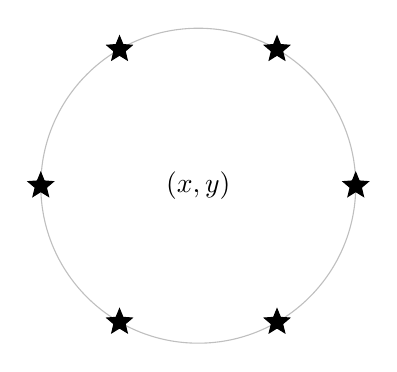
\begin{tikzpicture}
  % Central point
  \node at (0,0) {$(x,y)$};

  % Draw a circle to visualize the radial burst pattern
  \draw[lightgray] (0,0) circle (2cm); 

  % 6 stars positioned radially
  \foreach \angle in {0,60,...,300} {
    \node[star,star points=5,star point ratio=2.25, fill=black, inner sep=1.5pt,draw] at (\angle:2cm) {};
  }
\end{tikzpicture}

\end{document}
